\documentclass{journal}
\usepackage[utf8]{inputenc}
\usepackage{multicol}
\usepackage{graphicx}
\usepackage{amsmath}
\usepackage{amsfonts}
\usepackage{mathtools}
\usepackage{siunitx}
\usepackage{braket}
\usepackage{parskip}
\usepackage{wrapfig}
\usepackage{xparse,mathtools}
\usepackage{bm}
\usepackage[letterpaper, portrait, margin=1in]{geometry}
\renewcommand{\baselinestretch}{1.4}
\title{Quantum Homework 11}
\subtitle{PHY308 Spring 2019}
\author{Samuel Bellenchia}
\begin{document}
\maketitle
\section*{17.) Quantum v. Classical; }
%
Returning to problem 16's theme except from a new perscpective, we now determine if various systems are better approached classically or using quantum physics by the ratio of available thermal energy (given by $k_bT$) to the energy spacing of the system. So, for the following systems we're finding the ratio $k_bT/\Delta E$ \\

\textbf{a)} A particle on a ring is similar to a particle in a box in that it's movement is restricted by an infinite potential outside the path of it's orbit about a circle of radius $R_{moon}\approx3.8*10^8m$, the energy of such a system is $E_n=\frac{\hbar^2n^2}{2mR_{moon}^2}$ where the moon's mass $m_{moon}\approx7.34*10^{22}kg$. Assuming the smallest possible gap in energy, we take $\Delta E=E_2-E_1=\frac{4\hbar^2}{2mR^2}-\frac{\hbar^2}{2mR^2}=\frac{3\hbar^2}{2mR^2}\approx6.02*10^{-107}$.\\
We're given the temperature of the core to calculate the thermal energy, $T_{moon}=1700K$, so our ratio  $k_bT/E_{moon}\approx3.9*10^{86}$. As expected, this means $k_bT>>E_{moon}\Rightarrow$ \textit{very} classical system.\\

\textbf{b) } Now, we have the same system except at the scale of the Hydrogen atom, and we're taking the energy diffeence between the first excited state and the ground state, which is $\Delta E=E_1-E_2=-13.6eV-\frac{-13.6eV}{2^2}\approx10.2eV=1.63*10^{-18}J$.\\ At room temperature (~$295K$) our ratio of energy spacing to thermal energy is $\Delta E/K_bT=\frac{1.6*10^{-18}}{1.38*10^{-23}*295}\approx0.002498$.\\

Unsurprisingly, the ratio here is less than 1, meaning our system is best treated using quantum mechanics.\\

\textbf{c) } We are looking for the density of states in a metal at the Fermi energy, in order to find this formula, I referred to the following lecture notes from a University of Berlin course on semiconductor physics.\\
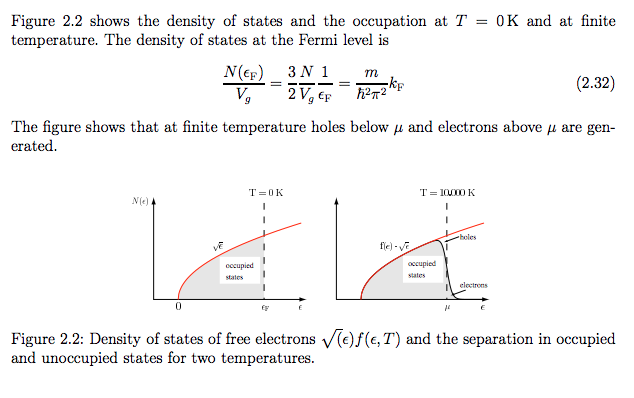
\includegraphics[width=\linewidth]{dos.png}\\

They've defined the density of states as $\frac{N}{V_g}=\frac32\frac{N}{V_g}\frac{1}{E_{\text{fermi}}}=\frac{m}{\hbar^2\pi^2}k_F$ and for metals  $k_F\approx2\AA^{-1}$. Since we're looking for ratio of thermal energy to the spacing in energy levels by virtue of the hint provided, we can multiply the states' density by $k_BT$ to get an estimate of the number of states populated, we get about $5.5*10^{20}$. The ratio then is $5.5*10^{20}/E_\text{fermi}=\frac{5.5*10^(20)}{1.85*10^{-18}}\approx3*10^{38}$\\

This is a huge ratio again, giving the intuitive result that in some cases, electrons do behave classically. Evidently, one of these cases is near the Fermi energy.\\

\textbf{d) } We're told to use the fluctuation in energy provided ("a 3.0GHz electron with $0.1\%$ energy spread.") So simply, our ratio of energy to spacing is $\frac{3*10^{9}Hz}{0.001*10^(9)Hz}=1000$.\\

Yet again, you can reasonably treat this system (electrons in a beam) with classical mechanics, despite the quantum scale of the particles in question.\\

\textbf{e) } Now, we examine a neutron in $^{56}{Fe}$ nucleus at room temperature, treating the nucleus as a "box."\\

We know the energy levels of a particle in a box are $E_n=\frac{\hbar^2\pi^2n^2}{2mL^2}$ where in our case, $L\approx7.5*10^{-15}m$ and $m=1.67*10^{-27}kg$. Again, we will take the smallest gap in energy, $\Delta E=E_2-E_1$\\

$k_bT/\Delta E=4*10^{-21}/(\dfrac{3\hbar^2\pi^2}{(1.67*10^{-27})*(7.5*10^{-15})^2})\approx5.82*10^{-11}$\\

In this case, our system in very, \textit{very} appropriate for the use of quantum mechanics.\\

\textbf{f) } We now deal with a proton in a beaker of acidic water vibrating at 80THz ($80*10^{12}Hz$). We know from our solution of the quantum harmonic oscillator that $E_n=\hbar\omega(n+\frac12)$, so the energy spacing is $\Delta E=\hbar\omega=(6.6*10^{-34})(80*10^{12})=8.43*10^{-21}$ and our thermal energy again is $295*k_b\approx4*10^{-21}$. So our ratio is;\\


$k_bT/\Delta E=4*10^{-21}/8.43*10^{-21}\approx0.5$.  Thus, this is a quantum system yet again.\\
\textbf{g) } We don't talk about part g...\\
\textbf{h) } The LIGO setup; a $40kg$ mass on a $0.5m$ silica fibre. This is a damped oscillator (damped due to air resistance) but ignoring friction, the frequency of oscillator for a pendulum in earth's gravitational field is; $\omega=\sqrt{\frac{g}{L}}=\sqrt{{9.8}{0.5}}=\sqrt{19.6}=4.42718$
, so our ratio is; $k_bT/\Delta E=4*10^{-21}/((4.43Hz)\hbar)\approx1.3*10^{12}$.\\

\textbf{i) } Similar to the previous system, we now have an atomoic force microscope vibrating at $100kHz$ at 1 Kelvin.\\

$\cfrac{1*k_b}{10^{8}\hbar}=1309.20296$, this is a system best treated classically.\\

\textbf{j) } The completed problem set actually exhibits a  material property known as energy manifestation, which arises due to the hardship undergone by the student completing it. The manifested energy is proportional to the cubic liters of human tears shed during the problem set's completion, divided by the number of assignments comprising the set.\\

The energy level is dependant on the number of your assignment, so we have $E_n={V_\text{tears}}/{n}$, however this is the equation in the vaccuum of empty space. For our system, the homework box of length 0.3m and height/width 0.1m (Volume $3*10^{-3}m^3$) tells us the energy levels are divided by the volume. This measurment is not precise but is convenient given the volume of tears is also $3*10^{-3}m^3$, I know this because I keep a graduated cyllinder by my desk to collect them.\\

For the lowest energy difference we then have $\Delta E=0.5$, and our ratio is $2*295*k_b$. This tells us that in the end, your homework isn't actually quantum at all. In fact, you wake up from your dream where you studied Physics in undergrad and realize you're pursuing an associates degree in Gender Studies at your local community college.

%
%
%
%
%
\pagebreak
%_____________________________________________________________________%
%_____________________________________________________________________%
\section*{36.) Two Particles in a box}
%_____________________________________________________________________%
%_____________________________________________________________________%
Two electrons are in a 1D square well with collision potential given by $V(x_1,x_1)=A\delta(x_1-x_2)$\\
%_____________________________________________________________________%
\textbf{a) Assume A=0 and solve for ground state wave function and Energy;}\\
%_____________________________________________________________________%

In one dimension, Schrodinger's equation for the infinite square well potential is as follows;\\
$\frac{-\hbar^2}{2m}\frac{d^2}{dx^2}\psi=E\psi\Rightarrow\psi^{''}(x)+\frac{2mE}{\hbar^2}\psi(x)=0\Rightarrow\psi(x)=Ae^{ik_0x}+Be^{-ik_0x}$. Then, applying our first boundary conditions $\psi(0)=0\Rightarrow A=-B$ which means $\psi(x)=A_0sin(k_0x)$ and the latter condition $\psi(L)=0\Rightarrow sin(kL)=0$ imposes the constraint $k=\frac{n\pi}{L}$, so our result is $\psi(x)=A_0sin(\frac{n\pi x}{L})$. Thus, by solving $\hat{H}\ket{\psi_n}=E_n\ket{\psi_n}$ we have the eigenfunctions;
\begin{center}
$\psi_n(x)=\sqrt{\frac2L}sin(\frac{n\pi x}L)$,  with corresponding eigenvalues;  $E_n=\frac{\hbar^2\pi^2n^2}{2mL^2}$\\
\end{center}
This is because the solution must be \textit{symmetric} for Bosons and \textit{anti-symmetric} for Fermions, as in $\psi(x_1,x_2)=\pm\psi(x_2,x_1)$.  But when incorporating the Spinor $\bm{\chi}(s)$, we are required that the \underline{entire} wavefunction (both spacial and Spinor part) be symmetric/antisymmetric.

\begin{center}
\small
  ( Without spin, $\frac{\sqrt2}{L}(sin\frac{\pi x_1}{L}sin\frac{2\pi x_2}{L}-sin\frac{2\pi x_1}{L}sin\frac{\pi x_2}{L})$ is the ground state.)\\
\end{center}

Spin considered, our ground state should have minimal angular momenta, \textbf{s}=0, and consequentially \textbf{m}=0. To find the coefficients of $\ket{0,0}=c_1\ket{\frac{\pm1}{2},\frac{\mp1}{2}}+c_2\ket{\frac{\mp1}{2},\frac{\pm1}{2}}$ we use the Clebsch-Gordan table, and obtain this superposition of spin up/down ($m_{i}=\frac12$/$\frac{-1}2$) states;
\begin{center}
$\ket{0,0}=\frac{1}{\sqrt{2}}[\ket{\uparrow\downarrow}-\ket{\downarrow\uparrow}]$\\
\end{center}
Our particles can occupy the same energy level if their overall (spin included) states differ, telling us the ground state has $n_1=1$,$n_2=1$. This spin state is antisymmetric, meaning it must be coupled with a symmetric spacial wavefunction. This means we use the symmetric form of $\psi(n_1,n_2)=\psi_1(n_1)\psi_2(n_2)\pm\psi_1(n_2)\psi_2(n_1)$. (without spin this is reserved for bosons)\\

The ground state solution (in the form $\Psi=\psi(n_1n_2)\chi(m_1m_2)$ ) and corresponding energy is;\\
\begin{center}
\large
$\ket{\Psi}=\frac{2}{L}\text{sin}(\frac{\pi}{L}x_1)\text{sin}(\frac{\pi}{L}x_2)[\frac{\sqrt{2}}2\ket{\uparrow\downarrow}-\frac{\sqrt{2}}2\ket{\downarrow\uparrow}]$, with $E_{11}=\frac{\hbar^2\pi^2}{2mL^2}(n_1^2+n_2^2)=\frac{\hbar^2\pi^2}{mL^2}$\\
\end{center}
\pagebreak
%_____________________________________________________________________%
\textbf{b) Find the first order correction our ground state energy}\\
%_____________________________________________________________________%

This is given by $E_1^{(1)}=\braket{\psi_1^{(0)}|\hat{H}^{'}|\psi_1^{(0)}}$, so for $\hat{H}^{'}=A\delta(x_1-x_2)$ our integral becomes;\\
\begin{center}
$ {\displaystyle\int_0^L}{\displaystyle\int_0^L}\text{sin}^2(\frac\pi{L}x_1)\text{sin}^2(\frac\pi{L}x_2)\delta(x_1-x_2)dx_1dx_2 $\\
\end{center}
I then searched for Trigonometric identities, Fourier series, Taylor's expansions, etc. but found nothing I could use. Finally, choosing; $x_m=x_1-x_2$ and $x_p=x_1+x_2$ I found;\\
\begin{center}

$ {\displaystyle\int_{-L}^L}{\displaystyle\int_0^{2L}}\text{sin}^2(\frac{\pi(x_m+x_p)}{2L})\text{sin}^2(\frac{\pi(x_p-x_m)}{2L})\delta(x_m)dx_pdx_m $\\

\end{center}
Now, the following graphic shows the input/output of my program computing this;\\
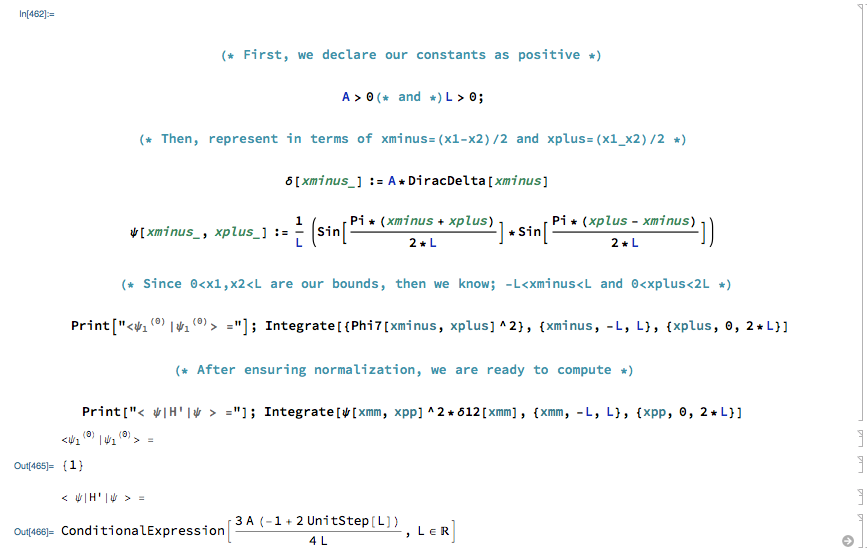
\includegraphics[width=1.1\linewidth]{ABC.png}\\
UnitStep[L]=1 since we $L\geq0$, and since $[A]=length*energy$, our energy correction is;\\
\begin{center}
\large
    $E_{1}^{(1)}=\braket{\psi_1^{(0)}|\hat{H}^{'}|\psi_1^{(0)}}=\frac{3A(-1+2)}{4L}=\frac{3A}{4L}$
\end{center}
\pagebreak
%_____________________________________________________________________%
\textbf{c) With A=0 what are the possible first excited states?}\\
%_____________________________________________________________________%
Firstly, notice the spacial solutions have multiple eigenfunctions (shown below) with corresponding energies $E_{n_1n_2}$ in the first excited state, since if either particle occupies $n_i=2$, by our formula
$E_{n_1n_2}=\frac{\hbar^2\pi^2}{2mL^2}(n_1^2+n_2^2)$ either state  yields the same value,  $E_{12}=E_{21}=\frac{5\hbar^2\pi^2}{2mL^2}$, where
\begin{center}
$\psi_{12}(x_1,x_2)=\frac{\sqrt2}{L}(sin\frac{\pi x_1}{L}sin\frac{2\pi x_2}{L}-sin\frac{2\pi x_1}{L}sin\frac{\pi x_2}{L})=-\psi_{21}$\\    
\end{center}

Next, let's examine the spin degeneracy of the first excited state, $\bm{s}=1$. We know our spin angular momentum operators, total 
$\hat{\bm{S}}^2\ket{\psi}=\hbar^2 s(s+1)\ket{\psi}$ and the z component
$\hat{\bm{S}}_z\ket{\psi}=\hbar m_s\ket{\psi} $ define numbers s and $m_s$ such that $m_s=-s,..,s$. So, $s=1\Rightarrow m_s=-1,0,1$ and we have three possible states in the $\ket{s_1s_2,m_1m_2}$ basis
\begin{center}
    $\ket{1,1}=\ket{\frac{1}{2}\frac{1}{2}\frac{1}{2}\frac{1}{2}}=\ket{\uparrow\uparrow}\text{ }\text{ }\text{ , and }\text{ }\text{ }\ket{1,-1}=\ket{\frac{1}{2}\frac{1}{2}\frac{-1}{2}\frac{-1}{2}}=\ket{\downarrow\downarrow}\text{ }\text{ }\text{ , and }\text{ }\text{ }\ket{1,0}=\frac{1}{\sqrt{2}}(\ket{\uparrow\downarrow}+\ket{\downarrow\uparrow})$\\
\end{center}
If not for the spacial part, the first and last of these would violate Putin's Collusion Principle,  but electrons with different energy levels can have the same $m_s$ values. Our great leader simply states two electrons cannot have identical sets of quantum numbers. To make our lives easier, I am adopting the following notation $\ket{n_1n_2sm}=\psi(n_1n_2)\chi(s,m)$, so I'll never have to write these functions again after this. Finally;\\
\begin{center}
$\ket{1210}=\frac{\sqrt2}{L}(sin\frac{\pi x_1}{L}sin\frac{2\pi x_2}{L}-sin\frac{2\pi x_1}{L}sin\frac{\pi x_2}{L})\frac{1}{\sqrt{2}}(\ket{\uparrow\downarrow}+\ket{\downarrow\uparrow})$\\
.\\

$\ket{1211}=\frac{\sqrt2}{L}(sin\frac{\pi x_1}{L}sin\frac{2\pi x_2}{L}-sin\frac{2\pi x_1}{L}sin\frac{\pi x_2}{L})\ket{\uparrow\uparrow}$\\
.\\

$\ket{121 ^-1 }=\frac{\sqrt2}{L}(sin\frac{\pi x_1}{L}sin\frac{2\pi x_2}{L}-sin\frac{2\pi x_1}{L}sin\frac{\pi x_2}{L})\ket{\downarrow\downarrow}$\\
.\\

$\ket{2110}=\frac{\sqrt2}{L}(sin\frac{2\pi x_1}{L}sin\frac{\pi x_2}{L}-sin\frac{\pi x_1}{L}sin\frac{2\pi x_2}{L})\frac{1}{\sqrt{2}}(\ket{\uparrow\downarrow}+\ket{\downarrow\uparrow})$\\
.\\

$\ket{2111}=\frac{\sqrt2}{L}(sin\frac{2\pi x_1}{L}sin\frac{\pi x_2}{L}-sin\frac{\pi x_1}{L}sin\frac{2\pi x_2}{L})\ket{\uparrow\uparrow}$\\
.\\

$\ket{211 ^-1 }=\frac{\sqrt2}{L}(sin\frac{2\pi x_1}{L}sin\frac{\pi x_2}{L}-sin\frac{\pi x_1}{L}sin\frac{2\pi x_2}{L})\ket{\downarrow\downarrow}$\\
.\\
\end{center}

Those, are ALL the eigenfunctions of the ground state, each with $E=\frac{5\hbar^2\pi^2}{2mL^2}$. Note that the spinors are all symmetric under interchange, so only antisymmetric spacial functions are allowed.\\
%_____________________________________________________________________%
\textbf{d) Take A}$>$\textbf{0, after correction which of these will have the lowest energy?}\\
%_____________________________________________________________________%
The lowest energy should be $\ket{1210}$ because the z-component of spin angular momenta is 0.\\

Thanks for everything Gleb, the help you've provided throughout the semester does not go unappreciated.\\ 

I wish you the best, and aspire to some day have a fraction of as many papers with my name on it as you.\\ Jeez man, leave some work for the rest of us!

\end{document}